Dopo aver determinato il volume dei dati ed aver associato a ciascuna operazione principale richiesta la frequenza di esecuzione procediamo ad esaminare gli schemi di navigazione per le principali operazioni richieste.

\subsubsection*{u.1 Registrazione di un nuovo utente}
L'utente si registra inserendo i dati minimi richiesti, in seguito potrà aggiungere altri campi modificando il proprio profilo.
\begin{longtblr}
[
  caption = {Registrazione di un nuovo utente},
]{
  colspec = {|X[3]X[1]X[2]X[4]|},
  rowhead = 1,
  hlines,
  row{even} = {PaleTurquoise},
  row{1} = {SkyBlue},
} 
Concetto & Costrutto & Accessi & Tipo\\
Users & E & 1 & Scrittura \\
\SetCell[c=4]{l, white} {
  Totale: 1S \textrightarrow 300/giorno\\
  Costo totale: 300 x (1\thinspace x \thinspace 2) = 600/giorno
  }

\end{longtblr}


\subsubsection*{u2. Login di un utente}
Per consentire il login si controlla che la combinazione username/password sia corretta e che l'utente non sia bannato. 
\begin{longtblr}
[
  caption = {Login di un utente},
]{
  colspec = {|X[3]X[1]X[2]X[4]|},
  rowhead = 1,
  hlines,
  row{even} = {PaleTurquoise},
  row{1} = {SkyBlue},
} 
Concetto & Costrutto & Accessi & Tipo\\
Users & E & 1 & L\\ 
\SetCell[c=4]{l, white} {
  Totale: 1L \textrightarrow 1500/giorno\\
  Costo totale: 1500 x (1) = 1500/giorno
  }

\end{longtblr}

\subsubsection*{u3. Modificare i dati del proprio account}
L'utente modifica i propri dati oppure inserisce quelli mancanti.
\begin{longtblr}
  [
    caption = {Modificare i dati del proprio account},
  ]{
    colspec = {|X[3]X[1]X[2]X[4]|},
    rowhead = 1,
    hlines,
    row{even} = {PaleTurquoise},
    row{1} = {SkyBlue},
  } 
  Concetto & Costrutto & Accessi & Tipo\\
  Users & E & 1 & S\\ 
  \SetCell[c=4]{l, white} {
  Totale: 1S \textrightarrow 300/giorno\\
  Costo totale: 300 x (1 \thinspace x \thinspace 2) = 600/giorno
  }
  \end{longtblr}

%%%%%%%%%%%%%%%%%%%%
%%%%%% ADMIN %%%%%%%
%%%%%%%%%%%%%%%%%%%%
\subsubsection*{a1. Consultare la lista degli utenti}
L'amministratore può visualizzare gli utenti registrati e bannarli o riattivarli all'occorrenza.
\begin{longtblr}
  [
    caption = {Consultare la lista degli utenti},
  ]{
    colspec = {|X[3]X[1]X[2]X[4]|},
    rowhead = 1,
    hlines,
    row{even} = {lightgray},
    row{1} = {LightCoral},
  } 
  Concetto & Costrutto & Accessi & Tipo\\
  User & E & 1 & L\\  
  ban & R & 1 & L\\ 
  \SetCell[c=4]{l, white} {
    Totale: 2L \textrightarrow 50/giorno\\
    Costo totale: 50 x (2) = 100/giorno
    }

  \end{longtblr}


  \subsubsection*{a2. Bannare gli altri utenti}
  Un amministratore banna un utente impedendone i futuri login.
  \begin{longtblr}
    [
      caption = {Bannare gli altri utenti},
    ]{
      colspec = {|X[3]X[1]X[2]X[4]|},
      rowhead = 1,
      hlines,
      row{even} = {lightgray},
      row{1} = {LightCoral},
    } 
    Concetto & Costrutto & Accessi & Tipo\\
    User & E & 1 & L\\
    ban & R & 1 & S \\ 

    \SetCell[c=4]{l, white} {
      Totale: 1L + 1S \textrightarrow 5/giorno\\
      Costo totale: 5 x (1 \thinspace + \thinspace 1 \thinspace x \thinspace 2) = 15/giorno
      }
  \end{longtblr}


\subsubsection*{a3. Reset delle recensioni}
In caso di necessità è possibile cancellare tutte le recensioni di un ente.
\begin{longtblr}
[
caption = {Reset delle recensioni},
]{
colspec = {|X[3]X[1]X[2]X[4]|},
rowhead = 1,
hlines,
row{even} = {lightgray},
row{1} = {LightCoral},
} 
Concetto & Costrutto & Accessi & Tipo\\
Ente & E & 1 & L \\
vendita & R & 1 & L \\
Servizio & E & 8 & L\\ 
Servizio & E & 8 & S\\ 
Recensione & R & 1600 (200 x 8) & L \\
Recensione & R & 1600 & S \\

\SetCell[c=4]{l, white} {
    Totale: 1610L + 1608S \textrightarrow 1/giorno\\
    Costo totale: 1 x (1610 \thinspace + \thinspace 1608 \thinspace x \thinspace 2) = \num{4826}/giorno
    }
\end{longtblr}



\subsubsection*{a4. Consultare le statistiche}
Verranno eseguite le query necessarie per ottenere le seguenti statistiche:\\
\begin{itemize}
  \item numero check-in
  \item numero check-in falliti
  \item numero CityCard attive
  \item numero eventi attivi
  \item numero servizi attivi
\end{itemize}
\begin{longtblr}
[
caption = {Consultare statistiche},
]{
colspec = {|X[3]X[1]X[2]X[4]|},
rowhead = 1,
hlines,
row{even} = {lightgray},
row{1} = {LightCoral},
} 
Concetto & Costrutto & Accessi & Tipo\\
checkin{\_}completato & R & 1 & L \\
checkin{\_}falliti & R & 2 & L \\
possesso{\_}CityCard & R & 1 & L \\
vendita & R & 1 & L \\
organizzazione & R & 1 & L \\

\SetCell[c=4]{l, white} {
    Totale: 5L \textrightarrow 50/giorno\\
    Costo totale: 50 x (5) = 250/giorno
    }
\end{longtblr}


%%%%%%%%%%%%%%%%%%%%%%%%
%%%%%% FORNITORE %%%%%%%
%%%%%%%%%%%%%%%%%%%%%%%%

\subsubsection*{f1. Creare enti}
Ogni fornitore può creare uno o più enti.
\begin{longtblr}
[
caption = {Creare enti},
]{
colspec = {|X[3]X[1]X[2]X[4]|},
rowhead = 1,
hlines,
row{even} = {lightgray},
row{1} = {ColdPurple},
} 
Ente & E & 1 & S \\
crea{\_}ente & R & 1 & S \\
\SetCell[c=4]{l, white} {
Totale: 2S \textrightarrow 8/giorno\\
Costo totale: 8 x (2 \thinspace x \thinspace 2) = 32/giorno
}
\end{longtblr}


\subsubsection*{f2. Associarsi a un ente}
Il fornitore si può associare a un solo ente.
\begin{longtblr}
[
caption = {Associarsi a un ente},
]{
colspec = {|X[3]X[1]X[2]X[4]|},
rowhead = 1,
hlines,
row{even} = {lightgray},
row{1} = {ColdPurple},
} 
Concetto & Costrutto & Accessi & Tipo\\
lavoro & R & 1 & S \\ 
\SetCell[c=4]{l, white} {
    Totale: 1S \textrightarrow 3/giorno\\
    Costo totale: 3 x (1 \thinspace x \thinspace 2) = 6/giorno
    }
\end{longtblr}

\subsubsection*{f3. Creare servizi}
Ogni fornitore associato ad un ente può creare servizi.
\begin{longtblr}
[
caption = {Creare servizi},
]{
colspec = {|X[3]X[1]X[2]X[4]|},
rowhead = 1,
hlines,
row{even} = {lightgray},
row{1} = {ColdPurple},
} 
Concetto & Costrutto & Accessi & Tipo\\
vendita & R & 1 & S \\
Servizio & E & 1 & S \\
lavoro & R & 1 & L \\
\SetCell[c=4]{l, white} {
    Totale: 1L + 1S \textrightarrow 10/giorno\\
    Costo totale: 10 x (1 \thinspace + \thinspace 2 \thinspace x \thinspace 2) = 50/giorno
    }
\end{longtblr}


\subsubsection*{f4. Creare eventi occasionali}
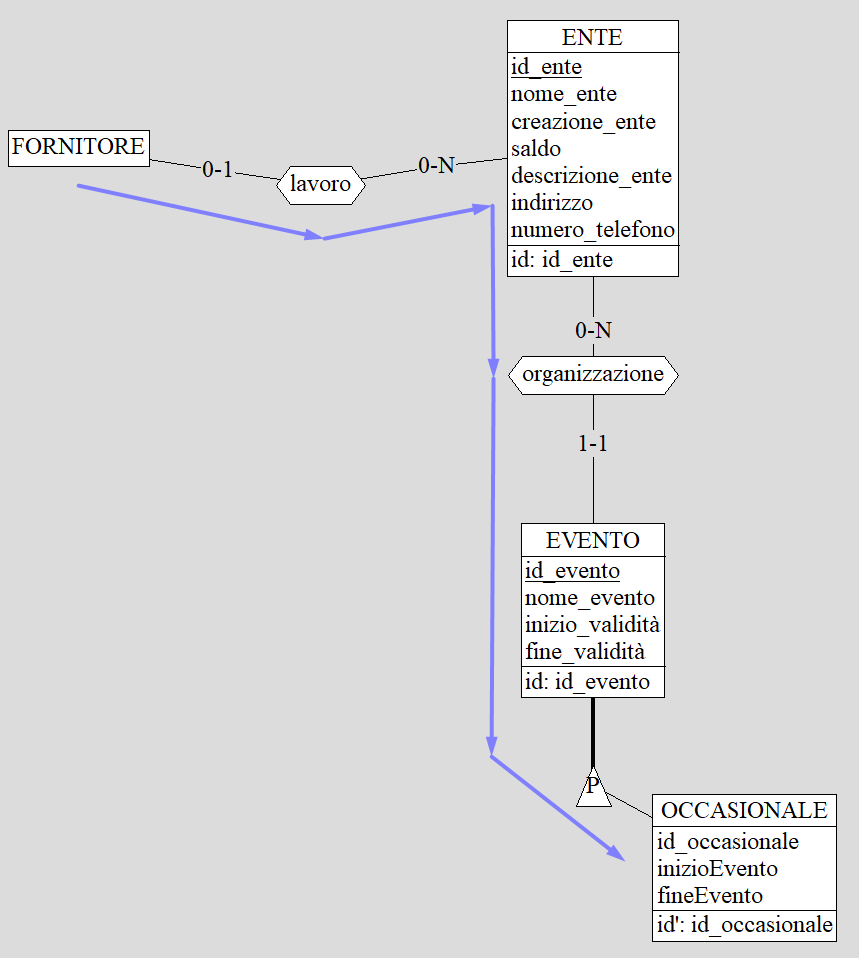
\includegraphics[width=0.95\columnwidth]{f4creaEventoOccasionale.png}\\
I fornitori associati a un ente possono creare eventi occasionali.
\begin{longtblr}
[
caption = {Creare eventi occasionali},
]{
colspec = {|X[3]X[1]X[2]X[4]|},
rowhead = 1,
hlines,
row{even} = {lightgray},
row{1} = {ColdPurple},
} 
Concetto & Costrutto & Accessi & Tipo\\
lavoro & R & 1 & L \\
organizza & R & 1 & S \\
Evento & E & 1 & S \\
Occasionale & E & 1 & S \\
\SetCell[c=4]{l, white} {
    Totale: 1L + 3S \textrightarrow 4/giorno\\
    Costo totale: 4 x (1 \thinspace + \thinspace 3 \thinspace x \thinspace 2) = 28/giorno
    }
\end{longtblr}




\subsubsection*{f5. Creare eventi periodici}
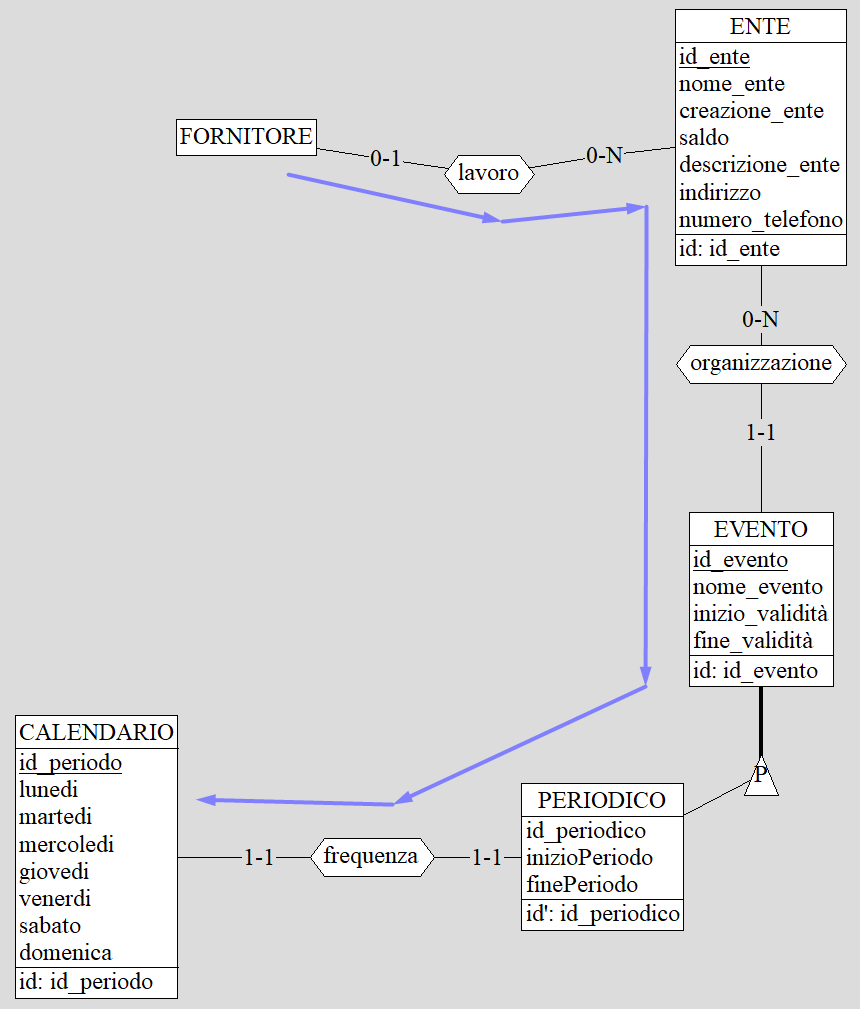
\includegraphics[width=0.95\columnwidth]{f5creaEventoPeriodico.png}\\
Per creare un evento periodico si dovrà ottenere l'id dell'ente al quale è associato il fornitore, poi andare a creare un record per l'evento e un altro record per il periodo. \\
\begin{longtblr}
[
caption = {Creare eventi periodici},
]{
colspec = {|X[3]X[1]X[2]X[4]|},
rowhead = 1,
hlines,
row{even} = {lightgray},
row{1} = {ColdPurple},
} 
Concetto & Costrutto & Accessi & Tipo\\
lavoro & R & 1 & L \\
organizza & R & 1 & S \\
Evento & E & 1 & S \\
Periodico & E & 1 & L \\
frequenza & R & 1 & S \\
Calendario & E & 1 & S \\
\SetCell[c=4]{l, white} {
    Totale: 2L + 4S \textrightarrow 1/giorno\\
    Costo totale: 1 x (2 \thinspace + \thinspace 4 \thinspace x \thinspace 2) = 10/giorno
    }
\end{longtblr}



\subsubsection*{f6. Consultare statistiche riguardo il proprio ente}
Oltre alla query per ottenere l'id dell'ente del fornitore verranno eseguite quelle necessarie per ottenere le seguenti statistiche:\\
\begin{itemize}
  \item saldo dell'ente associato al fornitore
  \item numero eventi attivi
  \item numero servizi attivi
\end{itemize}

\begin{longtblr}
[
caption = {Consultare statistiche riguardo il proprio ente},
]{
colspec = {|X[3]X[1]X[2]X[4]|},
rowhead = 1,
hlines,
row{even} = {lightgray},
row{1} = {ColdPurple},
} 
Concetto & Costrutto & Accessi & Tipo\\
Ente & E & 1 & L \\
Eventi & E & 1 & L\\ 
Servizi & E & 1 & L\\ 
\SetCell[c=4]{l, white} {
    Totale: 2L \textrightarrow 800/giorno\\
    Costo totale: 800 x (3) = 2400/giorno
    }
\end{longtblr}

%%%%%%%%%%%%%%%%%%%%%%
%%%%%% CLIENTE %%%%%%%
%%%%%%%%%%%%%%%%%%%%%%
\subsubsection*{c1. Richiedere una CityCard}
Il cliente richiede una nuova CityCard.
\begin{longtblr}
[
caption = {Richiedere una CityCard},
]{
colspec = {|X[3]X[1]X[2]X[4]|},
rowhead = 1,
hlines,
row{even} = {lightgray},
row{1} = {MediumSeaGreen},
} 
Concetto & Costrutto & Accessi & Tipo \\
possesso{\_}cityCard & R & 1 & S \\
CityCard & E & 1 & S \\
\SetCell[c=4]{l, white} {
    Totale: 2S \textrightarrow 2000/giorno\\
    Costo totale: 2000 x (2 \thinspace x \thinspace 2) = 8000/giorno
    }
\end{longtblr}

\subsubsection*{c2. Sottoscrivere un abbonamento}
Prima di sottoscrivere un abbonamento vengono cercate una CityCard valida e una carta di credito predefinita. \\
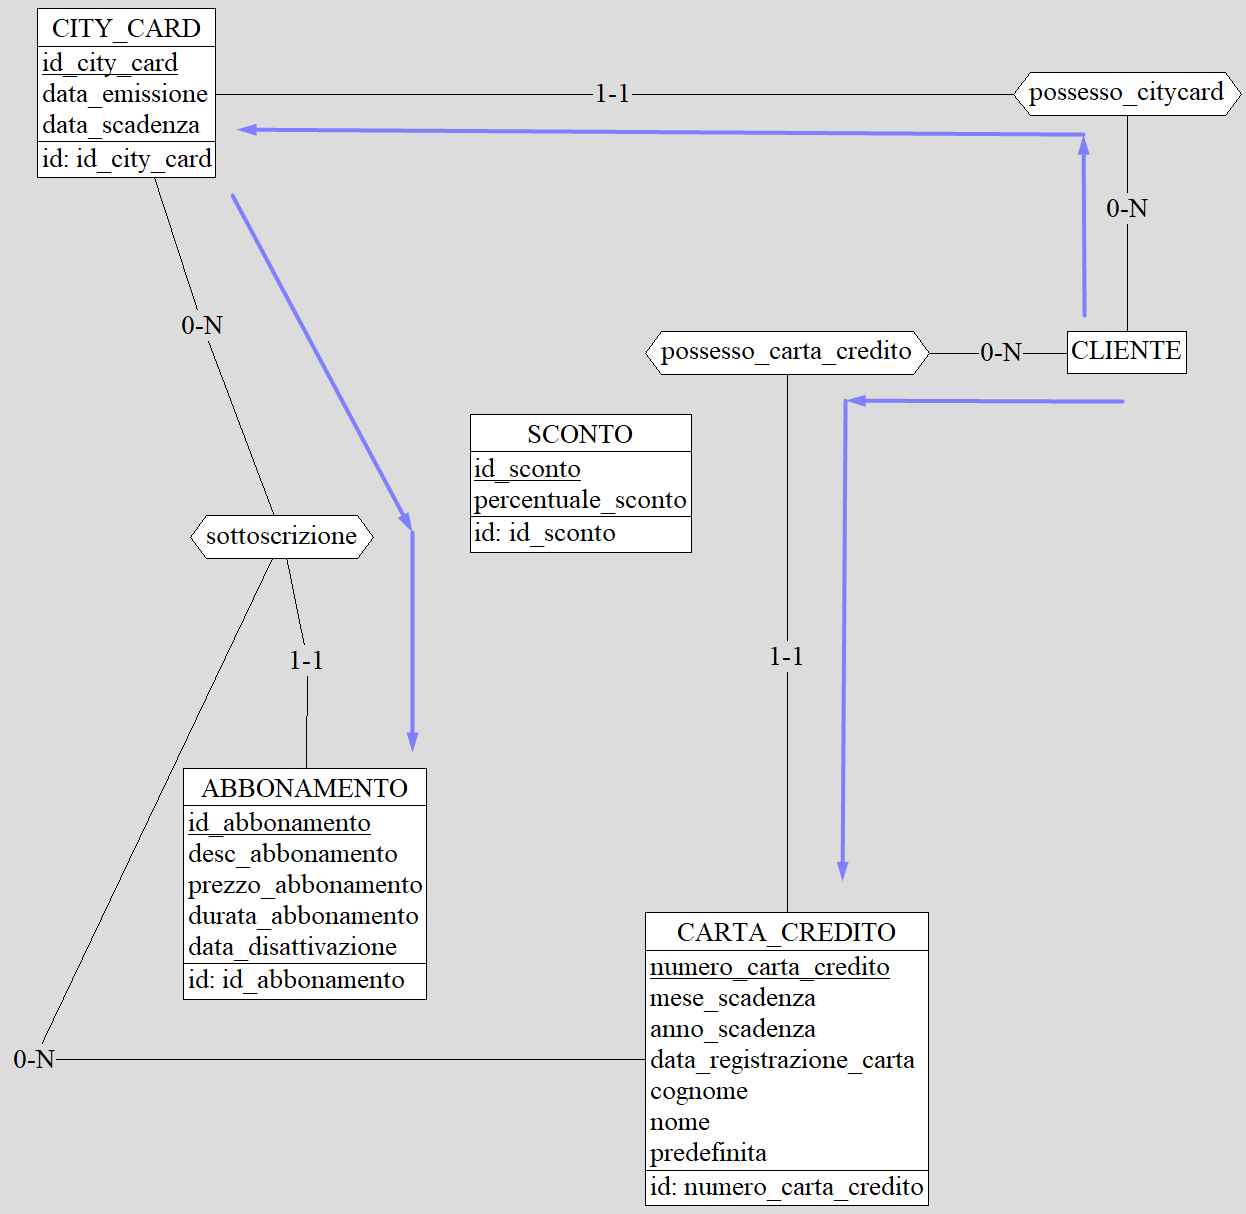
\includegraphics[width=0.95\columnwidth]{c2sottoscrizioneAbbonamento.png}\\

\begin{longtblr}
[
caption = {Sottoscrivere un abbonamento},
]{
colspec = {|X[3]X[1]X[2]X[4]|},
rowhead = 1,
hlines,
row{even} = {lightgray},
row{1} = {MediumSeaGreen},
} 
Concetto & Costrutto & Accessi & Tipo \\
Cliente & E & 1 & L\\ 
possesso{\_}carta{\_}credito & R & 1 & L \\
Carta{\_}Credito & E & 1 & L \\
possesso{\_}citycard & R & 1 & L \\
CityCard & E & 1 & L \\
sottoscrizione & R & 1 & S \\
\SetCell[c=4]{l, white} {
    Totale: 5L + 1S \textrightarrow 2000/giorno\\
    Costo totale: 2000 x (5 \thinspace + \thinspace 1 \thinspace x \thinspace 2) = 16000/giorno
    }
\end{longtblr}


\subsubsection*{c3. Aggiungere una carta di credito}
Un cliente può salvare le proprie carte di credito.
\begin{longtblr}
[
caption = {Aggiungere una carta di credito},
]{
colspec = {|X[3]X[1]X[2]X[4]|},
rowhead = 1,
hlines,
row{even} = {lightgray},
row{1} = {MediumSeaGreen},
} 
Concetto & Costrutto & Accessi & Tipo \\
Carta{\_}credito & R & S \\
possesso{\_}carta{\_}credito & R & 1 & S \\
\SetCell[c=4]{l, white} {
    Totale: 2S \textrightarrow 2000/giorno\\
    Costo totale: 2000 x (2 \thinspace x \thinspace 2) = 8000/giorno
    }
\end{longtblr}


\subsubsection*{c4. Rendere una carta di credito predefinita}
Rendo predefinita una carta di credito di un utente e non predefinite tutte le altre.\\
(dato che in media ho 1,5 carte per cliente, approssimo a 2)
\begin{longtblr}
[
caption = {Aggiungere una carta di credito},
]{
colspec = {|X[3]X[1]X[2]X[4]|},
rowhead = 1,
hlines,
row{even} = {lightgray},
row{1} = {MediumSeaGreen},
} 
Concetto & Costrutto & Accessi & Tipo \\
possesso{\_}carta{\_}credito & R & 2 & L \\
Carta{\_}credito & R & 2 & L \\
Carta{\_}credito & R & 2 & S \\
\SetCell[c=4]{l, white} {
    Totale: 4L + 2S \textrightarrow 2000/giorno\\
    Costo totale: 2000 x (4 \thinspace + \thinspace 2 \thinspace x \thinspace 2) = 16000/giorno
    }
\end{longtblr}


\subsubsection*{c5. Acquistare un servizio}
Viene controllata la CityCard dell'utente, tramite essa vengono recuperati i dati della sottoscrizione, poi quelli dello sconto, con questi dati viene calcolato il prezzo e infine viene comprato il servizio e aggiornato il saldo dell'ente.
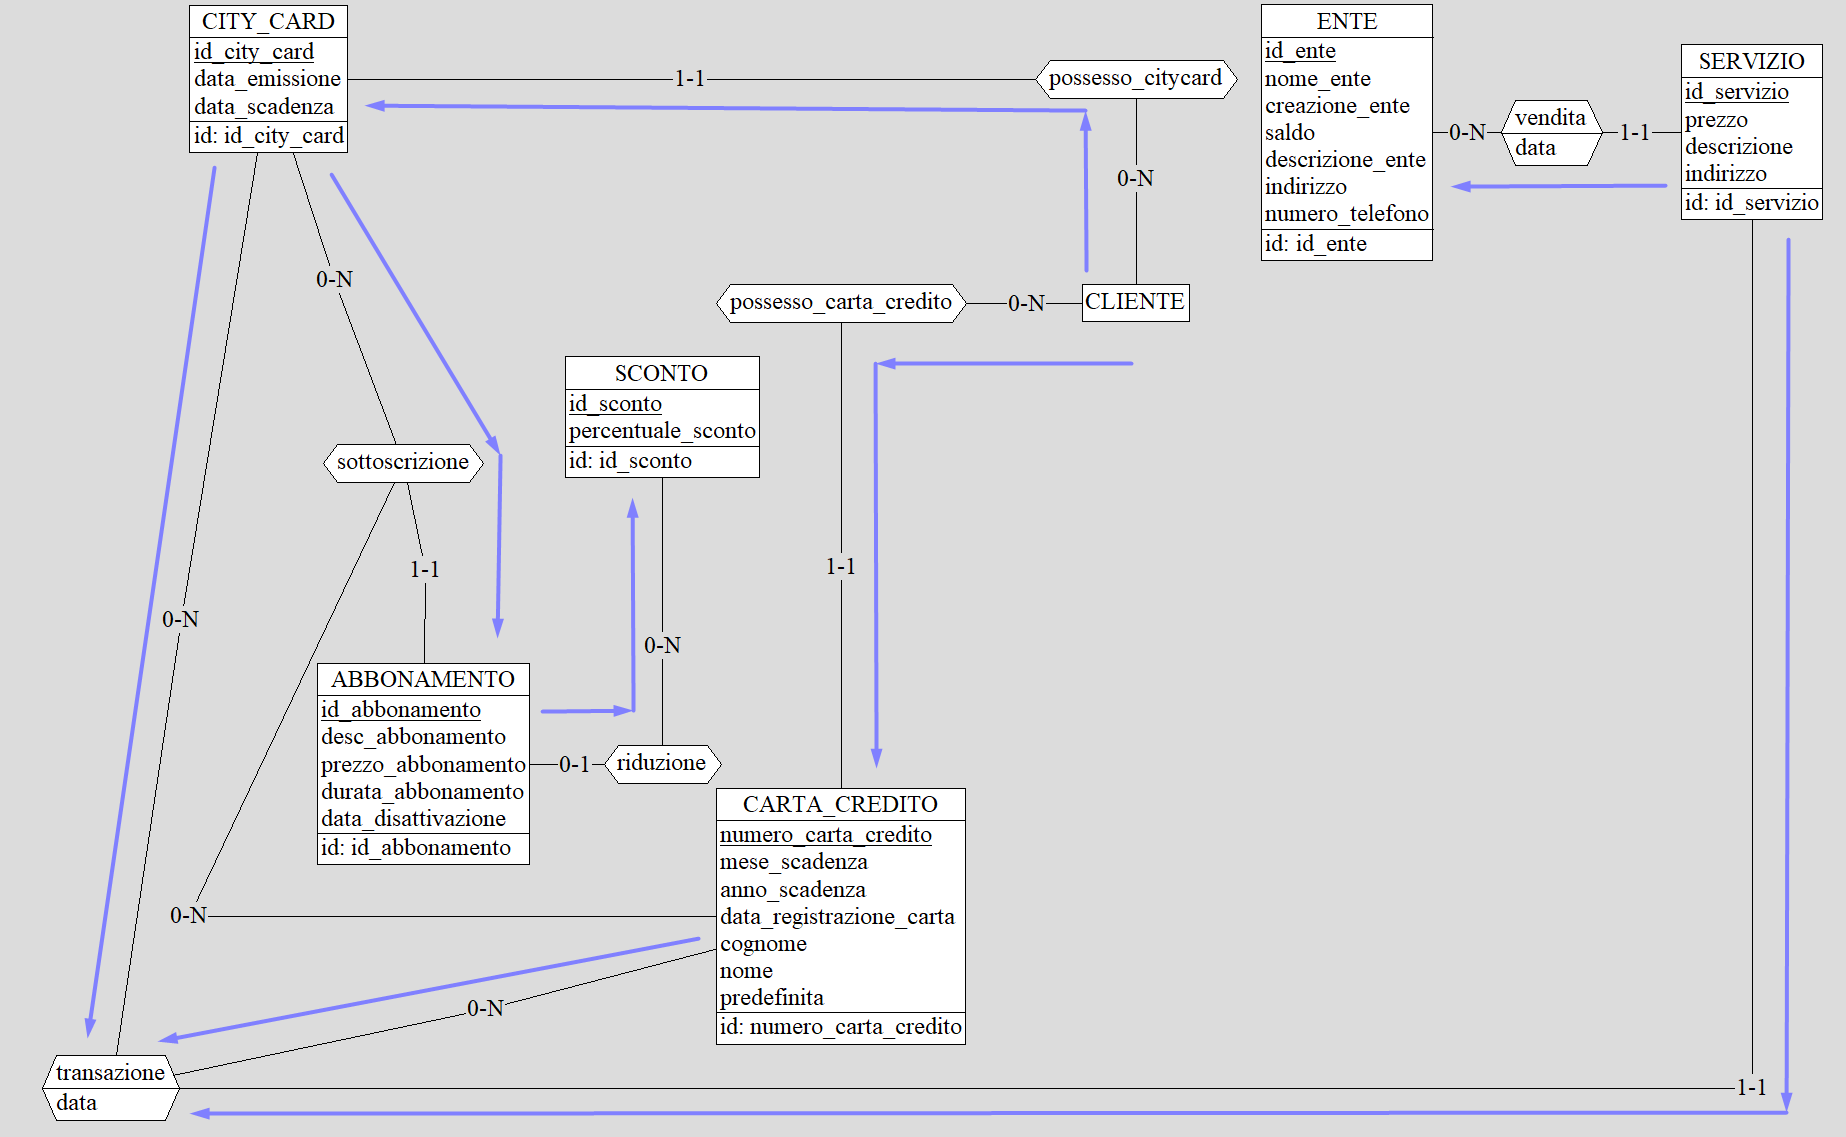
\includegraphics[width=0.95\columnwidth]{c5acquistaServizio.png}\\

\begin{longtblr}
[
caption = {Acquistare un servizio},
]{
colspec = {|X[3]X[1]X[2]X[4]|},
rowhead = 1,
hlines,
row{even} = {lightgray},
row{1} = {MediumSeaGreen},
} 
Concetto & Costrutto & Accessi & Tipo \\
possesso{\_}citycard & R & 1 & L \\
CityCard & E & 1 & L\\ 
sottoscrizione & R & 1 & L \\
Abbonamento & E & 1 & L\\ 
riduzione & R & 1 & L \\
Sconto & E & 1 & L\\ 
possesso{\_}carta{\_}credito & R & 1 & L \\
Carta{\_}credito & E & 1 & L \\
transazione & R & 1 & S\\ 
Servizio & E & 1 & L\\ 
vendita & R & 1 & L\\ 
Ente & E & 1 & S\\ 
\SetCell[c=4]{l, white} {
    Totale: 10L + 2S \textrightarrow 3000/giorno\\
    Costo totale: 3000 x (10 \thinspace + \thinspace 2 \thinspace x \thinspace 2) = 42000/giorno
    }
\end{longtblr}

\subsubsection*{c6. Prenotare un evento}
Gli utenti possono prenotare gratuitamente degli eventi.
\begin{longtblr}
[
caption = {Prenotare un evento},
]{
colspec = {|X[3]X[1]X[2]X[4]|},
rowhead = 1,
hlines,
row{even} = {lightgray},
row{1} = {MediumSeaGreen},
} 
Concetto & Costrutto & Accessi & Tipo \\
partecipazione{\_}persona & R & 1 & S \\
\SetCell[c=4]{l, white} {
    Totale: 1S \textrightarrow 500/giorno\\
    Costo totale: 500 x (1 \thinspace x \thinspace 2) = 1000/giorno
    }
\end{longtblr}


\subsubsection*{c7. Effettuare un check-in}
Per poter effettuare un check-in devo confermare che la CityCard del cliente sia valida.
\begin{longtblr}
[
caption = {Effettuare un check-in},
]{
colspec = {|X[3]X[1]X[2]X[4]|},
rowhead = 1,
hlines,
row{even} = {lightgray},
row{1} = {MediumSeaGreen},
} 
Concetto & Costrutto & Accessi & Tipo \\
possesso{\_}citycard & R & 1 & L \\
CityCard & E & 1 & L\\ 
checkin(completato/fallito) & R & 1 & S \\
\SetCell[c=4]{l, white} {
    Totale: 2L + 1S \textrightarrow 5000/giorno\\
    Costo totale: 5000 x (2 \thinspace + \thinspace 1 \thinspace x \thinspace 2) = 20000/giorno
    }
\end{longtblr}

\subsubsection*{c8. Consultare la lista degli acquisti fatti}
Un utente può visualizzare la lista di tutti gli acquisti fatti.
\begin{longtblr}
[
caption = {Consultare la lista degli acquisti fatti},
]{
colspec = {|X[3]X[1]X[2]X[4]|},
rowhead = 1,
hlines,
row{even} = {lightgray},
row{1} = {MediumSeaGreen},
} 
Concetto & Costrutto & Accessi & Tipo \\
possesso{\_}citycard & R & 1 & L \\
CityCard & E & 1 & L\\ 
transazione & R & 1 & L\\ 
\SetCell[c=4]{l, white} {
    Totale: 3L \textrightarrow 3000/giorno\\
    Costo totale: 3000 x (3) = 9000/giorno
    }
\end{longtblr}


\subsubsection*{c9. Lasciare una recensione riguardo un servizio acquistato}
Questa funzionalità verrà approfondita nella prossima sezione dedicata al calcolo delle ridondanze.

\subsubsection*{c10. Visualizzare lista servizi}
Anche questa funzionalità verrà approfondita nella prossima sezione dedicata al calcolo delle ridondanze.


\subsubsection*{c11. Visualizzare lista eventi}
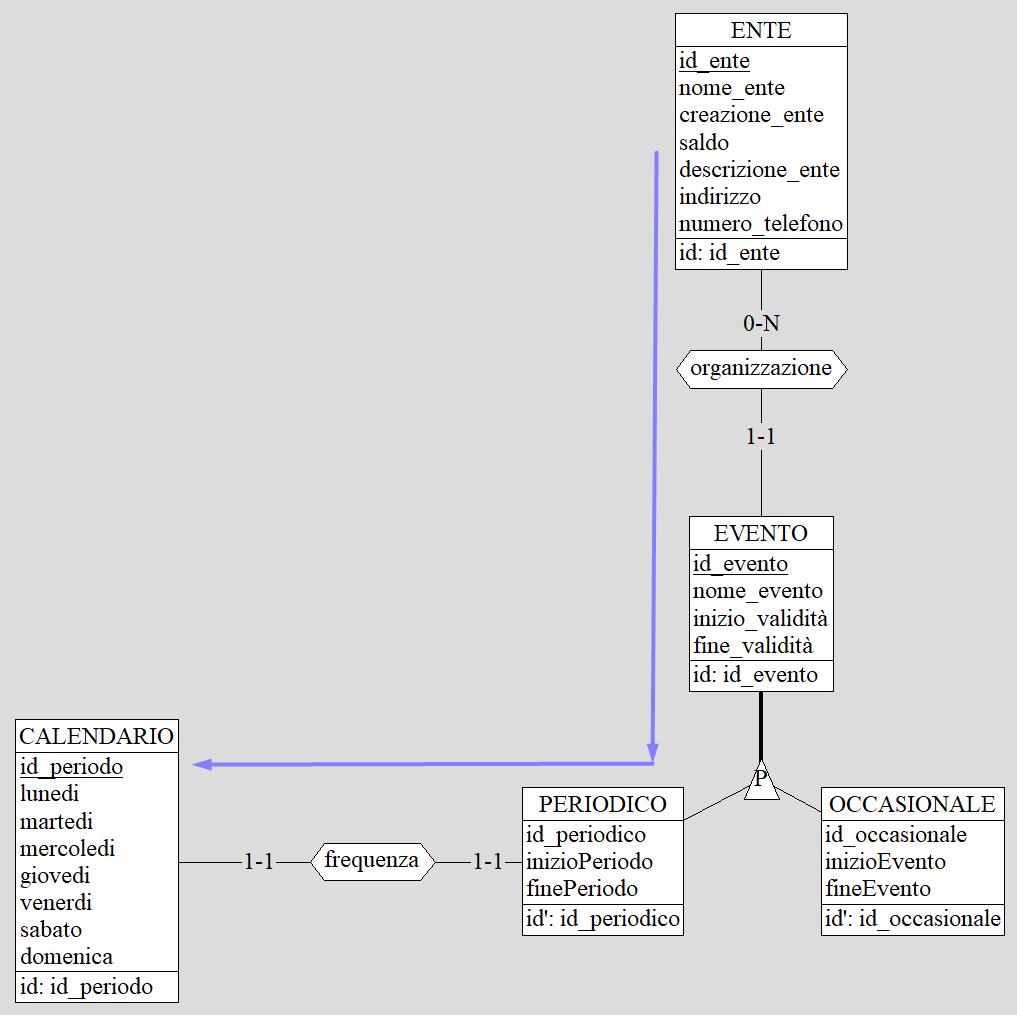
\includegraphics[width=0.95\columnwidth]{c11getEventi.png}\\
L'utente visualizza la lista di tutti gli eventi disponibili, sia periodici che occasionali.
\begin{longtblr}
[
caption = {Visualizzare lista eventi},
]{
colspec = {|X[3]X[1]X[2]X[4]|},
rowhead = 1,
hlines,
row{even} = {lightgray},
row{1} = {MediumSeaGreen},
} 
Concetto & Costrutto & Accessi & Tipo \\
Ente & E & 1 & L \\
organizzazione & R & 1 & L \\
Occasionale & E & 1 & L\\ 
Periodico & E & 1 & L\\ 
frequenza & R & 1 & L \\
Calendario & E & 1 & L\\ 

\SetCell[c=4]{l, white} {
    Totale: 6L \textrightarrow 1500/giorno\\
    Costo totale: 1500 x (6) = 9000/giorno
    }
\end{longtblr}
